\chapter{Procesamento automático das follas de tratamento}
\label{chap:procesamento-follas}

Unha das funcionalidades principais do sistema é a extracción automática da información contida nas follas de tratamento a partir dunha imaxe. O documento non está formado por texto continuo, senón que distribúe a información en diferentes seccións e táboas. Por este motivo, non é suficiente con recoñecer caracteres de maneira illada, tamén é necesario conservar a relación entre os campos e, especialmente, entre as datas e as doses da pauta diaria.

O procesamento destas follas presenta varias dificultades. En primeiro lugar, a información está organizada mediante campos illados, táboas, valores numéricos e representacións gráficas das doses. A táboa da pauta diaria resulta especialmente relevante, xa que os sistemas de recoñecemento poden identificar correctamente algúns dos seus elementos sen manter a organización en filas e columnas necesaria para asociar cada data coa súa dose.

En segundo lugar, existe unha variabilidade importante nas imaxes de entrada. O uso previsto da aplicación consiste en fotografar a folla mediante un dispositivo móbil, polo que a iluminación, a distancia, o encadramento ou a orientación poden variar entre capturas.

Finalmente, a información procesada é especialmente sensible. Un erro na identificación dunha data ou dunha dose podería provocar que a aplicación mostrase unha pauta incorrecta. Por este motivo, a capacidade de conservar correctamente a relación entre ambos elementos constitúe un dos principais criterios empregados durante a avaliación.

Co obxectivo de determinar unha aproximación adecuada para este problema, estudáronse diferentes técnicas de recoñecemento óptico de caracteres, detección de obxectos e procesamento documental. En concreto, avaliáronse Google ML Kit, Tesseract, unha aproximación baseada na combinación de YOLO cun motor OCR e dous tipos de modelos personalizados de Azure Document Intelligence. Ademais, desenvolveuse unha etapa de preprocesamento mediante OpenCV destinada a corrixir fotografías nas que a folla aparece inclinada ou deformada pola perspectiva.


% ============================================================
% MATERIAIS
% ============================================================

\section{Materiais}
\label{sec:materiais-procesamento}

\subsection{Conxunto de documentos}

Para realizar a experimentación recompilouse un conxunto formado por \textbf{11 follas de tratamento diferentes}. Antes de ser empregadas, eliminouse a información persoal que permitía identificar as persoas pacientes.

As follas manteñen unha estrutura xeral común, aínda que presentan variacións nos datos das visitas, nas datas, nas doses e na distribución dalgúns elementos. En particular, a táboa de doses pode conter representacións gráficas de fraccións de pastilla, valores numéricos e indicacións textuais como \textit{NO TOMAR} ou \textit{CONTROL}.

Cómpre diferenciar entre o número de documentos e o número de imaxes empregado durante as probas. O conxunto está formado por 11 follas diferentes, pero de cada unha delas obtivéronse varias imaxes en condicións distintas. Deste modo, foi posible estudar tanto o comportamento ante documentos diferentes como a influencia das condicións de captura sobre unha mesma folla.


\subsection{Condicións de captura}
\label{sub:cond-cap}

De cada unha das 11 follas obtivéronse \textbf{catro imaxes} baixo condicións de captura diferentes. Esta parte do conxunto está formada, polo tanto, por un total de \textbf{44 imaxes}.

As condicións consideradas foron as seguintes:

\begin{itemize}
    \item unha imaxe escaneada, considerada como caso ideal ou de referencia,
    \item unha fotografía realizada cunha iluminación adecuada,
    \item unha fotografía realizada cun nivel de iluminación inferior,
    \item unha fotografía tomada desde unha distancia maior, de forma que a folla ocupa unha proporción menor da imaxe.
\end{itemize}

Estas variacións pretenden representar situacións que poden producirse durante o uso real da aplicación, no que non se pode garantir que todas as fotografías se realicen cunha iluminación, distancia ou encadramento idénticos.

Adicionalmente, preparouse un subconxunto formado por \textbf{7 fotografías inclinadas}, correspondentes a sete das follas anteriores. Estas imaxes empregáronse especificamente para avaliar a etapa de preprocesamento encargada de corrixir a orientación e, cando é posible identificar os límites da folla, a perspectiva do documento.

Dentro deste subconxunto incluíronse \textbf{dúas fotografías cun fondo claro de tonalidade similar á propia folla}. O obxectivo destes casos foi introducir unha situación máis complexa para a detección do contorno, xa que unha diferenza reducida entre a cor do papel e a do fondo pode dificultar a súa delimitación.

En total, considerando as 44 imaxes correspondentes ás catro condicións de captura e as 7 fotografías inclinadas adicionais, o material preparado para a experimentación está formado por \textbf{51 imaxes obtidas a partir de 11 documentos base}.

A Táboa~\ref{tab:resumo-conxunto-imaxes} resume a composición deste conxunto.

\begin{table}[h!]
    \centering
    \caption{Resumo do conxunto de imaxes empregado na experimentación.}
    \label{tab:resumo-conxunto-imaxes}
    \begin{tabular}{lcc}
        \hline
        \textbf{Condición} &
        \textbf{Documentos} &
        \textbf{Imaxes} \\
        \hline
        Referencia & 11 & 11 \\
        Iluminación adecuada & 11 & 11 \\
        Baixa iluminación & 11 & 11 \\
        Maior distancia & 11 & 11 \\
        Inclinadas & 7 & 7 \\
        \hline
        \textbf{Total} & \textbf{11 diferentes} & \textbf{51} \\
        \hline
    \end{tabular}
\end{table}


\subsection{Distribución dos datos}

A utilización das imaxes variou segundo as necesidades de cada método. Google ML Kit e o modelo estándar de Tesseract non requiriron ningún proceso de adestramento, polo que se aplicaron directamente sobre os documentos seleccionados para cada proba. O conxunto concreto empregado en cada caso indícase posteriormente xunto cos seus resultados.

Nos métodos que si requiriron adestramento realizouse unha división a nivel de documento. As follas \textbf{F01--F08} destináronse ao adestramento, mentres que as follas \textbf{F09--F11} reserváronse exclusivamente para a avaliación. Esta mesma distribución empregouse no modelo personalizado de Tesseract, no detector baseado en YOLO e nos modelos personalizados de Azure Document Intelligence.

Deste modo, ningún exemplo procedente das follas F09--F11 foi empregado durante o adestramento, permitindo avaliar posteriormente os modelos sobre documentos non vistos previamente.

As fotografías inclinadas adicionais empregáronse especificamente para avaliar a etapa de preprocesamento mediante OpenCV.

%A preparación concreta dos datos foi diferente en cada caso. Para Tesseract, as oito follas de adestramento utilizáronse para obter recortes de liñas acompañados da súa transcrición correcta. No caso de YOLO, as imaxes correspondentes a estas follas etiquetáronse manualmente coas rexións que o detector debía localizar. Para Azure Document Intelligence, nas oito follas etiquetáronse os campos considerados de interese para o funcionamento da aplicación.. As tres follas reservadas mantivéronse fóra destes procesos de adestramento e empregáronse posteriormente para comprobar o comportamento sobre documentos non vistos.

% RECOMENDACIÓN:
% Identificar internamente as follas como F01, F02, ..., F11 facilita
% referencialas nas táboas e figuras posteriores.
%
% Por exemplo:
% F01-F08 -> adestramento.
% F09-F11 -> avaliación/proba.
%
% Se finalmente utilizas estes identificadores, mantelos iguais en todo
% o capítulo para poder asociar con claridade cada resultado coa imaxe correspondente.

% TODO:
% Aínda falta indicar o número exacto de recortes xerados para Tesseract
% e, se resulta relevante, o número total de anotacións realizadas en YOLO.


% ============================================================
% MÉTODOS
% ============================================================

\section{Métodos}
\label{sec:metodos-procesamento}

Nesta sección descríbense as diferentes aproximacións exploradas. O obxectivo é explicar o procedemento seguido con cada unha delas e a preparación dos datos necesaria.


% ------------------------------------------------------------
% ML KIT
% ------------------------------------------------------------

\subsection{Google ML Kit}

Para avaliar Google ML Kit, descrito na Sección~\ref{sec:tec-mlkit}, empregouse o seu módulo de recoñecemento de texto co obxectivo de comprobar se a saída xerada podía servir como base para interpretar automaticamente a folla de tratamento.

Desenvolveuse unha pequena aplicación en Flutter que permitía seleccionar unha imaxe almacenada no dispositivo ou capturar unha fotografía da folla e enviala ao recoñecedor de texto de ML Kit.

Como resultado, a ferramenta devolvía o texto detectado xunto coa súa organización en bloques, liñas e elementos. Esta información gardouse en formato JSON para facilitar a análise posterior da orde na que se devolvían os diferentes elementos do documento.

O proceso seguido pola aplicación represéntase na Figura~\ref{fig:secuencia-mlkit}.

\begin{figure}[h!]
    \centering
    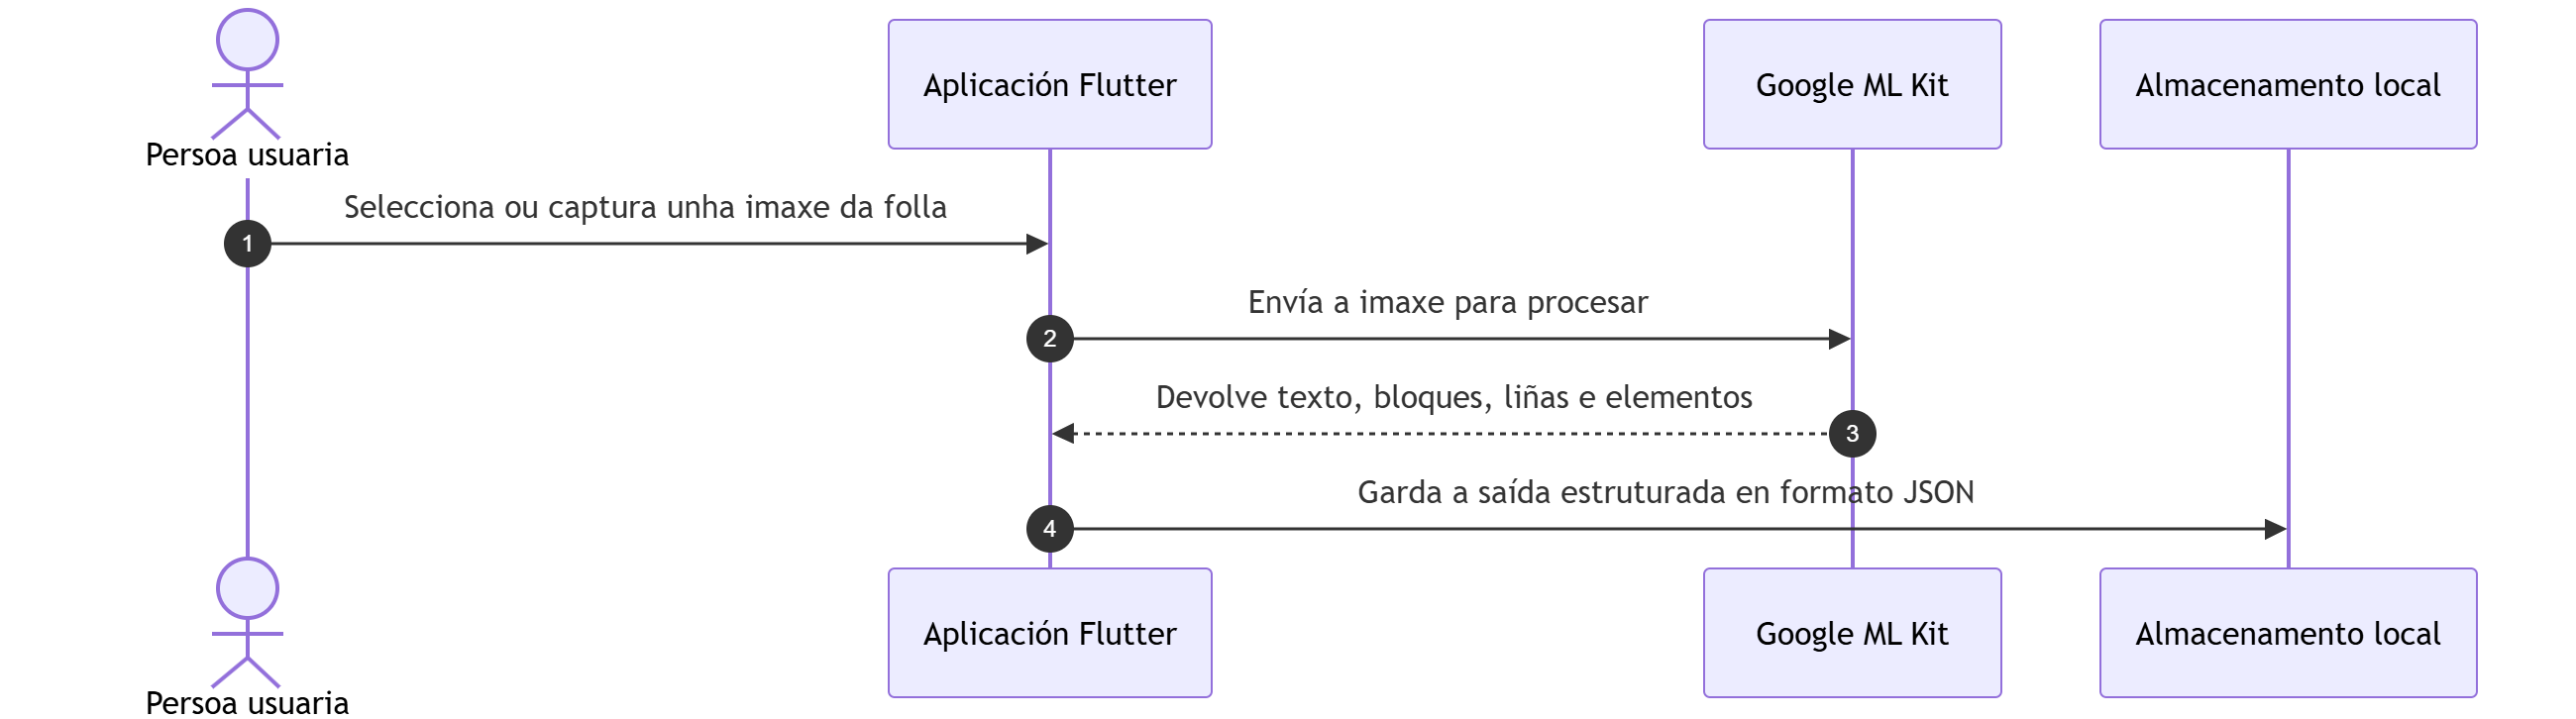
\includegraphics[width=0.9\linewidth]
    {imaxes/06-Procesamento automático das follas de tratamento/mermaid-mlkit.png}
    \caption{Secuencia seguida para procesar unha folla mediante Google ML Kit.}
    \label{fig:secuencia-mlkit}
\end{figure}


% ------------------------------------------------------------
% TESSERACT
% ------------------------------------------------------------

\subsection{Tesseract}

Para avaliar Tesseract, estudáronse dúas variantes, o modelo estándar para lingua española e un modelo personalizado adaptado ao tipo de documento empregado no proxecto.

A primeira proba realizouse empregando o modelo estándar de Tesseract para lingua española, sen introducir ningún proceso de adestramento adicional. As imaxes procesáronse como documentos completos e analizouse directamente a saída textual xerada polo motor OCR. O obxectivo desta proba foi comprobar se un sistema de recoñecemento de texto convencional era capaz de recuperar suficiente información da folla como para reconstruír posteriormente a súa estrutura.

Co obxectivo de adaptar Tesseract á tipografía, ao vocabulario e ao formato das follas de tratamento, construíuse un conxunto de adestramento específico.

Neste caso non se empregaron directamente documentos completos, senón recortes correspondentes a diferentes liñas das follas. Cada exemplo de adestramento estaba formado por dous ficheiros:

\begin{itemize}
    \item un ficheiro con extensión \textit{.png}, que contiña o recorte da liña;
    \item un ficheiro con extensión \textit{.gt.txt}, que contiña o \textit{ground truth}, é dicir, a transcrición correcta do texto presente na imaxe.
\end{itemize}

A partir destes pares realizouse o adestramento dun modelo denominado \textit{sintromv2}. O modelo non se adestrou desde cero, senón que se empregou como punto de partida o modelo español de Tesseract.

O proceso executouse mediante a ferramenta \textit{tesstrain}. O comando empregado foi:

\begin{verbatim}
make training MODEL_NAME=sintromv2 \
    START_MODEL=spa TESSDATA=../tessdata/
\end{verbatim}

Neste comando, \textit{MODEL\_NAME} indica o identificador do novo modelo, \textit{START\_MODEL} especifica o modelo de partida e \textit{TESSDATA} sinala o directorio no que se atopa o ficheiro \textit{spa.traineddata}.

Durante o proceso, \textit{tesstrain} emprega os pares formados pola imaxe e a súa transcrición para adaptar o modelo \gls{lstm} de Tesseract aos exemplos proporcionados.

% ------------------------------------------------------------
% YOLO
% ------------------------------------------------------------

\subsection{Detección de representacións de pastillas mediante YOLO}

A terceira aproximación estudada baseouse no uso de YOLO como detector de obxectos. A diferenza dun sistema OCR, este tipo de modelo non intenta interpretar directamente o texto da imaxe, senón localizar visualmente as rexións correspondentes ás clases que foron definidas durante o adestramento.

A aproximación formulouse en dúas fases. Na primeira, YOLO empregouse para localizar automaticamente as representacións gráficas das pastillas presentes na táboa da pauta. Na segunda, a posición obtida mediante o detector utilizouse como referencia para delimitar unha rexión máis ampla da cela e aplicar posteriormente OCR sobre ese recorte.

%A intención desta estratexia era reducir o problema observado nas aproximacións anteriores: en lugar de solicitar ao motor OCR que interpretase a folla completa e reconstruíse posteriormente a estrutura da táboa, intentábase primeiro localizar os elementos visuais máis característicos e limitar o recoñecemento de texto á súa contorna.

Para a preparación do detector empregouse a ferramenta CVAT, mediante a cal se etiquetaron manualmente as representacións gráficas das pastillas. Esta anotación realizouse baixo unha única clase denominada \textit{pastilla}, debuxando unha caixa delimitadora (bounding box) arredor de cada representación visual. Na Figura~\ref{fig:yolo-cvat} móstrase un exemplo deste proceso.

\begin{figure}[h!]
    \centering
    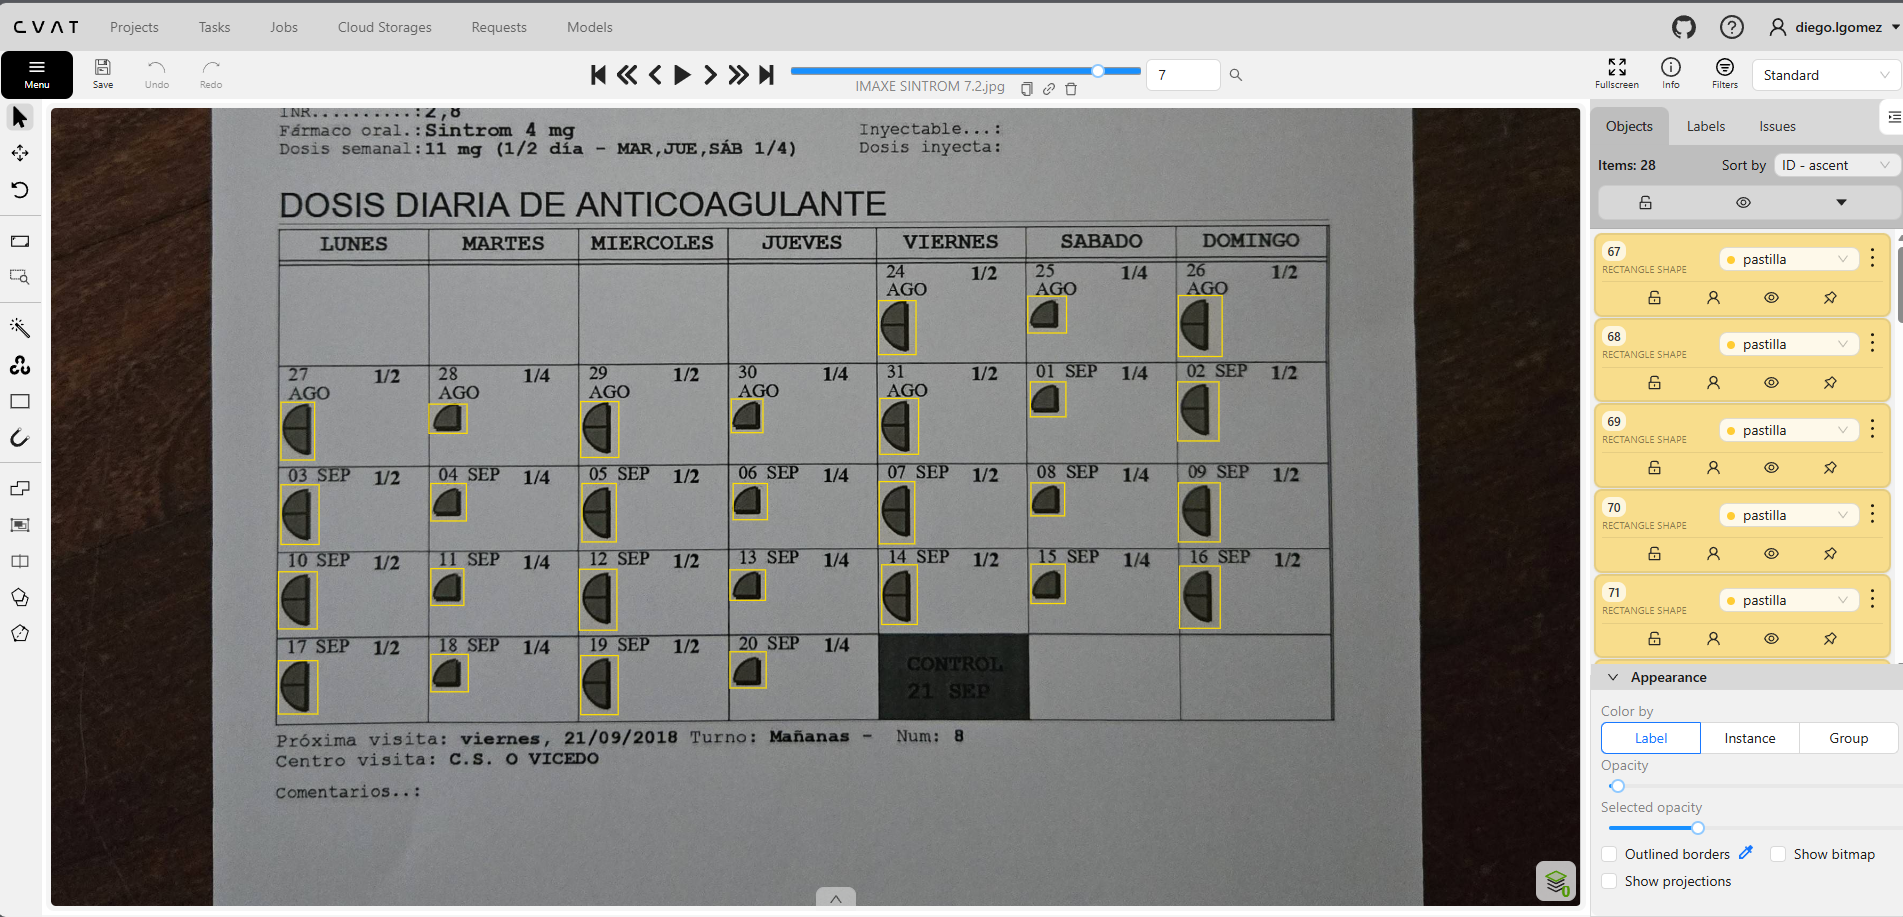
\includegraphics[width=0.85\textwidth]{imaxes/06-Procesamento automático das follas de tratamento/etiquetaxe-CVAT.png}
    \caption{Exemplo de etiquetaxe realizada en CVAT para a detección da clase \textit{pastilla}.}
    \label{fig:yolo-cvat}
\end{figure}

A partir deste conxunto de datos adestrouse un modelo denominado \textit{sintrom\_pastilla}, tomando como punto de partida o modelo preadestrado \textit{yolo11n.pt}. O comando empregado foi:

\begin{verbatim}
yolo detect train data=dataset_pastilla\data.yaml model=yolo11n.pt \
imgsz=1024 epochs=100 batch=4 name=sintrom_pastilla
\end{verbatim}

%Empregouse un tamaño de imaxe de 1024 píxeles debido ao reducido tamaño das representacións das pastillas dentro da folla de tratamento.

Unha vez obtida a detección, ampliouse a rexión delimitada polo modelo para intentar incluír tamén a información asociada á cela e aplicar un OCR sobre o recorte resultante.

Esta segunda fase presenta unha dificultade adicional, xa que a caixa detectada por YOLO corresponde unicamente á representación da pastilla e non aos límites reais da cela. Polo tanto, é necesario decidir canto debe ampliarse a rexión antes de aplicar OCR.

% TODO IMPORTANTE - YOLO + OCR:
%
% Tes que completar esta parte cando acabes as probas.
%
% Explicar:
% 1. Como amplías a bounding box da pastilla.
% 2. Que OCR aplicas finalmente ao recorte.
% 3. Exemplos nos que funciona.
% 4. Exemplos nos que a ampliación inclúe texto doutras celas.
%
% O problema que xa observaches é:
% - a pastilla detéctase ben;
% - ao ampliar a caixa para obter data/dose/cela,
%   ás veces entra información das celas veciñas;
% - ese texto adicional introduce ruído no OCR.
%
% NON concluír aínda aquí se funciona ou non.
% Iso vai na sección de resultados.


% ------------------------------------------------------------
% AZURE DOCUMENT INTELLIGENCE
% ------------------------------------------------------------

\subsection{Azure Document Intelligence}

Para avaliar Azure Document Intelligence optouse por adestrar modelos personalizados capaces de interpretar a estrutura específica das follas de tratamento. 

A partir das necesidades da aplicación definiuse un esquema cos campos que se consideraron relevantes para a extracción, entre eles as datas e doses da pauta diaria, o INR, o fármaco, a seguinte visita e a información correspondente ao histórico de visitas.

Estes campos etiquetáronse manualmente mediante Azure Document Intelligence Studio, asociando en cada documento as rexións correspondentes coas etiquetas definidas no esquema. Na Figura~\ref{fig:etiquetaxe-azure} móstrase un exemplo deste proceso.

\begin{figure}[h!]
    \centering
    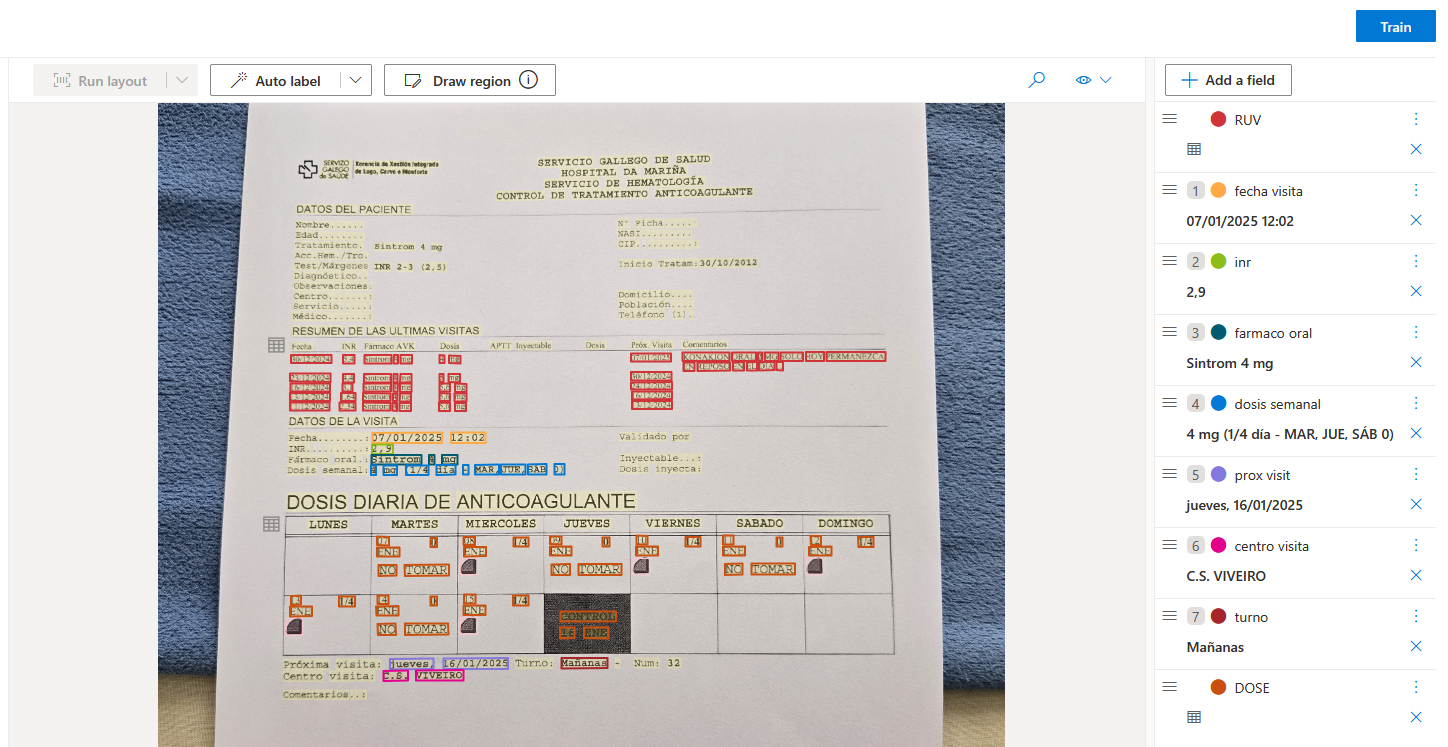
\includegraphics[width=0.9\textwidth]{imaxes/06-Procesamento automático das follas de tratamento/EtiquetaxeAzure.png}
    \caption{Interface de etiquetaxe en Azure Document Intelligence Studio.}
    \label{fig:etiquetaxe-azure}
\end{figure}

A partir do mesmo conxunto de documentos etiquetados adestráronse dous modelos personalizados, empregando as arquitecturas \textit{Neural} e \textit{Template}. A primeira está baseada en técnicas de aprendizaxe profunda e está orientada a documentos nos que a disposición e a posición da información poden variar entre exemplos. Esta maior flexibilidade implica tamén unha maior necesidade de datos de adestramento.

Pola súa banda, a arquitectura \textit{Template} baséase principalmente na disposición espacial dos elementos e na repetición de estruturas e patróns xeométricos entre os documentos, polo que está especialmente orientada a formatos cunha organización relativamente estable.

Dado o reducido número de documentos dispoñibles para o adestramento e a estrutura repetitiva das follas de tratamento, adestráronse e avaliáronse ambas arquitecturas co obxectivo de comparar o seu comportamento sobre o mesmo conxunto de datos.

As \textbf{3 follas reservadas para a avaliación}, que non foran empregadas durante o adestramento, utilizáronse para comparar ambas arquitecturas. Deste modo, os dous modelos puideron ser avaliados sobre os mesmos documentos e sobre información non vista previamente.

%METER ICUAL EN IMPLEMENTACION 
\subsection{Preprocesamento das imaxes mediante OpenCV}
\label{sec:preprocesamento-opencv}

Ademais das aproximacións estudadas para a extracción da información, incorporouse unha etapa previa de preprocesamento mediante OpenCV destinada a corrixir as fotografías nas que a folla aparece inclinada ou deformada pola perspectiva. Esta etapa non realiza a extracción dos datos, senón que prepara a imaxe antes de enviala ao sistema encargado do seu procesamento.

O procedemento deseñouse seguindo un criterio conservador: a imaxe só se modifica cando se detecta cun nivel suficiente de confianza que é necesaria unha corrección. En caso contrario, mantense a imaxe orixinal para evitar que unha transformación incorrecta poida eliminar ou deformar información relevante.

O proceso comeza coa detección dos bordos e dos principais contornos da imaxe, tratando de identificar a folla como unha rexión cuadrangular. Tamén se contempla unha segunda estratexia baseada na detección de superficies claras, pensada para fotografías nas que os límites do papel resultan menos evidentes. Cando se localizan de maneira fiable os catro extremos da folla, aplícase unha transformación de perspectiva que permite obter unha vista frontal do documento e eliminar parte do fondo exterior.

Se non é posible delimitar completamente a folla, emprégase unha alternativa baseada na orientación das liñas detectadas no documento. A partir delas estímase o ángulo de inclinación e, cando a desviación é significativa, rótase a fotografía para aliñala. Se non existe suficiente evidencia para aplicar ningunha das dúas correccións, a entrada continúa sen modificacións.

Esta etapa integrouse antes do proceso de extracción da API, de forma que o sistema encargado de interpretar o documento recibe a versión corrixida cando é necesario. Para avaliar especificamente este mecanismo preparouse un subconxunto de \textbf{7 fotografías inclinadas}, correspondentes a sete documentos diferentes. Dúas delas realizáronse sobre fondos claros similares á propia folla co obxectivo de comprobar o comportamento da detección en condicións de menor contraste.

% FIGURA RECOMENDADA:
% Nos resultados, mostrar:
% (a) imaxe inclinada orixinal;
% (b) resultado corrixido;
% (c) imaxe sobre fondo claro;
% (d) resultado correspondente.


% ============================================================
% CRITERIOS DE AVALIACIÓN
% ============================================================

\section{Criterios de avaliación}
\label{sec:criterios-avaliacion-procesamento}

Unha vez descritas as diferentes aproximacións, establecéronse os aspectos empregados para analizar os resultados obtidos e determinar a súa adecuación ao problema.

A avaliación centrouse principalmente nos seguintes criterios:

\begin{itemize}
    \item a capacidade de recoñecer correctamente texto, datas e valores numéricos;
    \item a conservación da estrutura das táboas;
    \item a asociación entre cada data e a súa dose correspondente;
    \item a estabilidade e facilidade de interpretación do formato de saída;
    \item o esforzo necesario para preparar e etiquetar os datos;
    \item o comportamento ante diferentes condicións de captura.
\end{itemize}

A táboa de doses considerouse o elemento máis importante da avaliación, xa que constitúe a base a partir da cal a aplicación representa a pauta diaria e programa os avisos correspondentes. Por este motivo, non se considerou suficiente que unha tecnoloxía recoñecese correctamente palabras ou números de maneira independente. Para resultar adecuada debía ser posible determinar de forma fiable que dose correspondía a cada data.

No caso da aproximación baseada en YOLO, valorouse adicionalmente a capacidade de localizar as representacións gráficas das pastillas e a posibilidade de utilizar esas deteccións como punto de partida para delimitar a información da cela correspondente.

No caso concreto da etapa de preprocesamento mediante OpenCV, a avaliación centrouse en comprobar se era posible detectar unha inclinación significativa, endereitar correctamente o documento e, cando se identificaban os seus catro bordos, corrixir tamén a deformación de perspectiva e recortar as zonas exteriores innecesarias.

Ao mesmo tempo, considerouse especialmente importante comprobar que unha fotografía xa correctamente aliñada non fose modificada e que, ante unha detección dubidosa, se mantivese a imaxe orixinal en lugar de aplicar unha transformación potencialmente incorrecta.

%REVISAR
Finalmente, unha vez seleccionada unha aproximación para realizar a extracción, avaliouse de forma específica o seu comportamento ante diferentes condicións de iluminación e distancia, xa que estas situacións representan mellor o contexto real no que se utilizará a aplicación.


% ============================================================
% RESULTADOS
% ============================================================

\section{Resultados}
\label{sec:resultados-procesamento}

\subsection{Resultados de Google ML Kit}

A avaliación de Google ML Kit realizouse inicialmente sobre as \textbf{11 follas de tratamento escaneadas}, consideradas como o escenario de referencia e as condicións máis favorables de entrada. O obxectivo desta primeira proba foi comprobar se a ferramenta permitía recuperar non só o texto presente no documento, senón tamén a información necesaria para reconstruír de maneira fiable a pauta de tratamento.

ML Kit conseguiu recoñecer unha parte importante do contido dos documentos. Non obstante, observáronse erros mesmo nestas condicións favorables. Entre os exemplos atopamos, valores de INR como \textit{1,9} e \textit{2,2} foron devoltos como \textit{19} e \textit{22}, respectivamente, e producíronse tamén modificacións en datas, como \textit{11/12/2024} recoñecido como \textit{1/12/2024} ou \textit{25/05/2018} como \textit{2.5/05/2018}.

% FONTES:
% F01.json -> INR 1,9 -> 19
% F10.json -> INR 2,2 -> 22
% F05.json -> 11/12/2024 -> 1/12/2024
% F07.json -> 25/05/2018 -> 2.5/05/2018

A principal limitación atopada apareceu na táboa de doses diarias. A ferramenta recoñece numerosos elementos do seu contido, pero a saída non conserva de maneira estable a estrutura visual da táboa. Entre as distintas imaxes probadas, as entradas aparecen agrupadas parcialmente por columnas ou distribuídas entre bloques diferentes, de modo que o día, o mes e a dose dunha mesma cela non sempre forman unha única secuencia. Como consecuencia, a orde textual obtida non coincide necesariamente coa orde cronolóxica da pauta. Por exemplo, nalgúns casos a dose aparece despois da data, como en \textit{20 DIC 1/4}, noutros sitúase antes, como en \textit{1/4 17 DIC} e tamén se observaron agrupacións como \textit{18 DIC 1/4 19 1/4 DIC}, nas que quedan mesturados elementos pertencentes a entradas distintas.


Esta variabilidade dificulta establecer un formato de saída sobre o que aplicar de maneira fiable patróns ou expresións regulares. As coordenadas proporcionadas por ML Kit poderían empregarse como apoio para reorganizar espacialmente os elementos detectados, pero non resolven os erros producidos no propio recoñecemento. Entre as follas escaneadas atopáronse, por exemplo, \textit{05 ENE} devolto como \textit{0 ENE}, doses \textit{1/2} recoñecidas como \textit{/2} e \textit{16 NOV} interpretado como
\textit{l6 NOV}. Nestes casos parte da información orixinal foi omitida ou substituída, polo que non pode recuperarse de maneira inequívoca mediante unicamente a reorganización dos elementos ou un postprocesamento.

% FONTES:
% F08.json -> 05 ENE -> 0 ENE
% F10.json -> 16 NOV -> l6 NOV
% F10.json -> aparecen doses 1/2 incompletas como /2

Unha vez identificadas estas limitacións nas imaxes de referencia, realizáronse probas adicionais con \textbf{cinco fotografías tomadas con iluminación normal}, co obxectivo de comprobar o comportamento da ferramenta nun escenario máis próximo ao uso real da aplicación. Os problemas estruturais mantivéronse, as entradas da pauta non sempre se devolveron seguindo a súa orde cronolóxica, senón agrupadas parcialmente por columnas e intercaladas con información procedente doutras zonas do documento.

Ademais, continuaron producíndose erros no propio contido recoñecido. Na pauta diaria apareceron repetidamente doses \textit{1/2} devoltas como \textit{/2} ou \textit{12}; tamén se modificaron días, como \textit{11 SEP} recoñecido como \textit{TI SEP}, e nalgún caso chegou a omitirse completamente o número do día, conservándose unicamente o mes e a dose. Fóra da táboa observáronse igualmente erros en campos, como \textit{Sintrom 4 mg} recoñecido como \textit{Sin tromn 4 ng}, así como modificacións en datas e valores numéricos, como \textit{15/01/2025} recoñecido como \textit{JS/01/2025} ou \textit{3,5 mg} como \textit{35 mg}.

% FONTES:
%
% F01-N.json:
% - orde da táboa alterada, con entradas agrupadas parcialmente por columnas
% - 08 SEP 1/2 -> 08 SEP /2
% - 11 SEP 1/2 -> TI SEP 1/2
% - 12 SEP 1/2 -> 12 SEP 12
% - 14 SEP 1/2 -> 14 SEP 12
% - 10 OCT 1/2 -> non se recoñece o número 10; quedan OCT e a dose
%
% F03-N.json:
% - Sintrom 4 mg -> Sin tromn 4 ng
% - 15/01/2025 -> JS/01/2025
% - 3,5 mg -> 35 mg
%
% F07-N.json:
% - tamén aparecen doses 1/2 recoñecidas como /2

A Figura~\ref{fig:mlkit-f01n-entrada} mostra un fragmento dunha das cinco fotografías tomadas con iluminación normal empregadas nestas probas, mentres que o Listing~\ref{lst:mlkit-f01n-saida} recolle a saída bruta xerada por ML Kit para esa mesma imaxe. Nel poden observarse de forma conxunta a perda da estrutura da táboa e os erros de recoñecemento descritos anteriormente.

\begin{figure}[hp!]
    \centering
    % Empregar F01-N.
    % RECOMENDACIÓN: recortar desde
    % "DOSIS DIARIA DE ANTICOAGULANTE"
    % ata o final da primeira fila (08--14 SEP).
    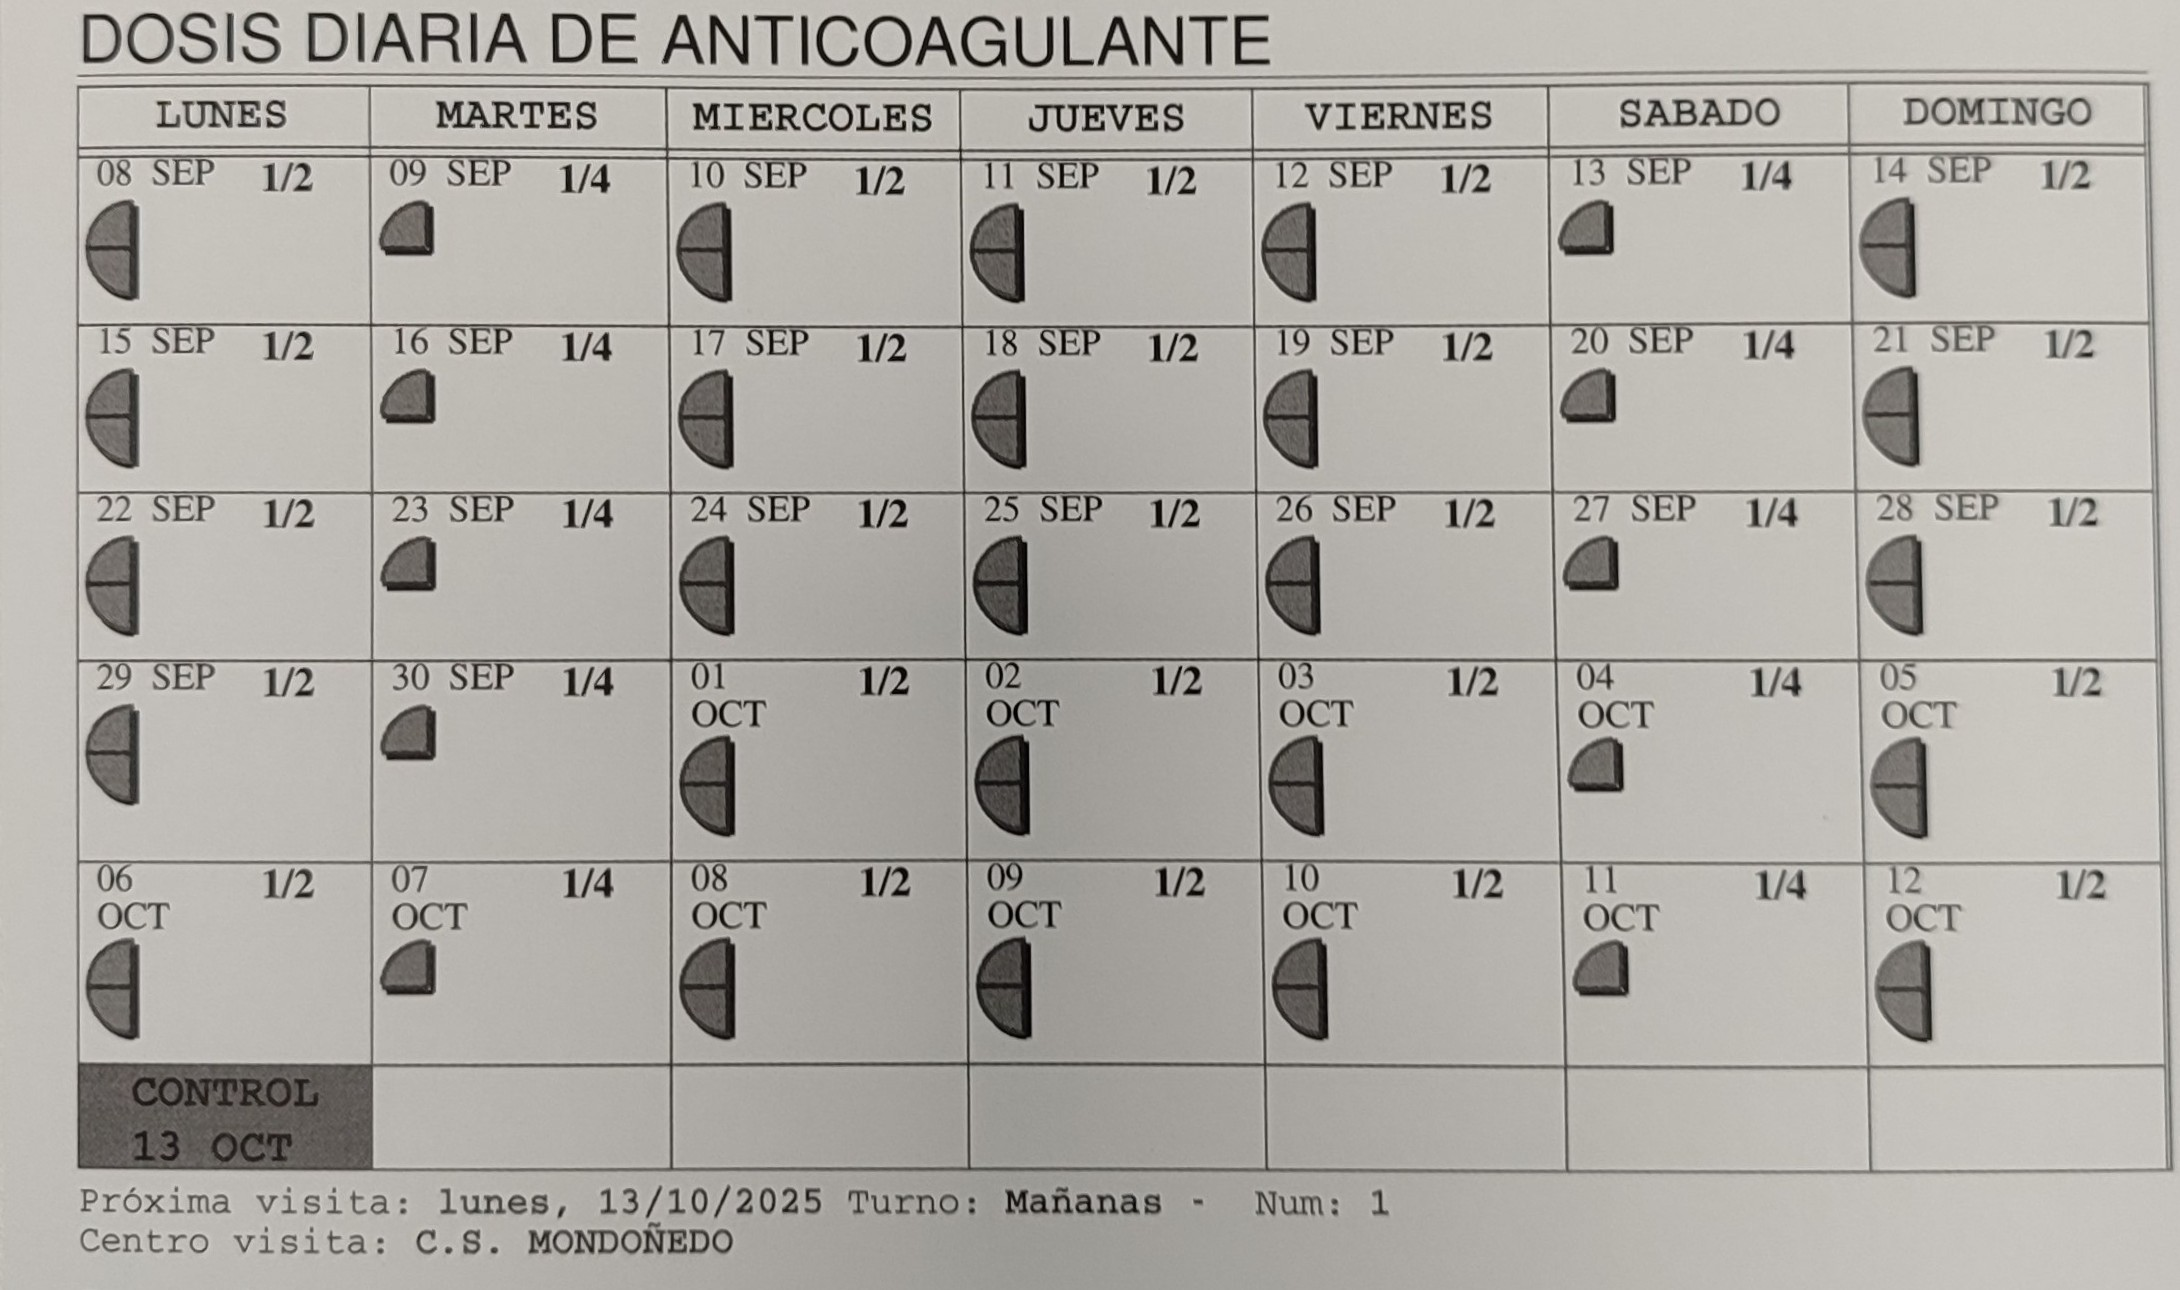
\includegraphics[width=0.75\textwidth]{imaxes/06-Procesamento automático das follas de tratamento/mlkit-f01n-pauta.jpg}
    \caption{Fragmento dunha fotografía tomada con iluminación normal
    empregada na avaliación de Google ML Kit.}
    \label{fig:mlkit-f01n-entrada}
\end{figure}

\begin{lstlisting}[
    frame=single,
    rulecolor=\color{gray!60},
    backgroundcolor=\color{gray!5},
    basicstyle=\ttfamily\scriptsize,
    escapeinside={(*}{*)},
    caption={Fragmento anotado da saída bruta de ML Kit para a fotografía da Figura~\ref{fig:mlkit-f01n-entrada}},
    label={lst:mlkit-f01n-saida},
    captionpos=t,
    columns=fullflexible,
    keepspaces=true
]
VIERNES
(*\textcolor{red}{12 SEP 12}*)   (*\textcolor{red}{$\leftarrow$ 1/2 recoñecido como 12}*)
C.S. MONDONEDO      (*\textcolor{red}{$\leftarrow$ información allea á pauta}*)
19 SEP
26 SEP
03
OCT
(*\textcolor{red}{OCT}*)         (*\textcolor{red}{$\leftarrow$ falta o día 10}*)
Num: 1             (*\textcolor{red}{$\leftarrow$ información doutra zona}*)
1/2
1/2
1/2
1/2                 (*\textcolor{red}{$\leftarrow$ doses separadas das datas}*)

SABADO
13 SEP 1/4
20 SEP
27 SEP
04
OCT
11
OCT
1/4
1/4
1/4
1/4                 (*\textcolor{red}{$\leftarrow$ datas e doses en grupos distintos}*)

DOMINGO
(*\textcolor{red}{14 SEP 12}*)   (*\textcolor{red}{$\leftarrow$ 1/2 recoñecido como 12}*)
21 SEP
28 SEP
05
OCT
[...]
12
OCT
12
12
(*\textcolor{red}{/2}*)          (*\textcolor{red}{$\leftarrow$ perda do numerador}*)
12
\end{lstlisting}

As probas realizadas sobre as \textbf{11 follas escaneadas} e as \textbf{cinco fotografías tomadas con iluminación normal} permitiron avaliar o comportamento de ML Kit tanto en condicións favorables como nun escenario máis próximo ao uso real da aplicación. Os resultados obtidos en ambos os casos mostraron limitacións que afectaban directamente á información necesaria para reconstruír a pauta de tratamento. Por este motivo, non se considerou necesario ampliar a avaliación a outras condicións de captura, xa que a
evidencia recollida resultaba suficiente para descartar a ferramenta como solución principal.

En consecuencia, aínda que Google ML Kit mostrou unha boa capacidade para recoñecer unha parte importante do texto presente nas follas, non proporcionou unha saída suficientemente fiable para reconstruír de forma segura a pauta diaria. Por este motivo, a ferramenta foi descartada como solución principal para a extracción automática.


% ------------------------------------------------------------
% RESULTADOS TESSERACT
% ------------------------------------------------------------

\subsection{Resultados de Tesseract}

\subsubsection{Modelo estándar}

A avaliación do modelo estándar de Tesseract realizouse sobre as \textbf{11 follas de tratamento escaneadas}, empregando o modelo para español \textit{spa}. Ao tratarse das imaxes de referencia, estas probas permitiron analizar o seu comportamento nas condicións de entrada máis favorables antes de considerar escenarios de captura máis complexos.

Tesseract conseguiu recuperar correctamente unha parte do texto xeral dos documentos, especialmente cabeceiras, etiquetas e algúns campos das visitas. Non obstante, os resultados presentaron numerosos erros tipográficos, confusións entre caracteres e modificacións en valores numéricos. Estes problemas afectaron tamén á información relevante para o tratamento. Por exemplo, nunha das follas apareceron valores como \textit{35 me}, \textit{29}, \textit{54} ou \textit{44} en campos nos que os valores orixinais incluían unidades ou separadores decimais. 
% F03.txt

A maior dificultade apareceu novamente na táboa de doses diarias. Aínda que nalgúns documentos se recoñeceron correctamente varias entradas, o comportamento foi moi irregular entre as distintas follas. Observáronse perdas ou modificacións dos separadores das fraccións, días incorrectos, caracteres sen relación co contido da táboa e agrupacións que dificultan establecer a correspondencia entre cada data e a súa dose.

Un dos exemplos máis representativos obsérvase na folla F04. Como mostra o Listing~\ref{lst:tesseract-estandar-f04}, a saída conserva algúns elementos recoñecibles, pero introduce numerosos caracteres incorrectos e perde a estrutura necesaria para asociar de forma fiable cada data coa súa dose.

\begin{figure}[h!]
    \centering
    % Recorte da táboa da folla F01 escaneada.
    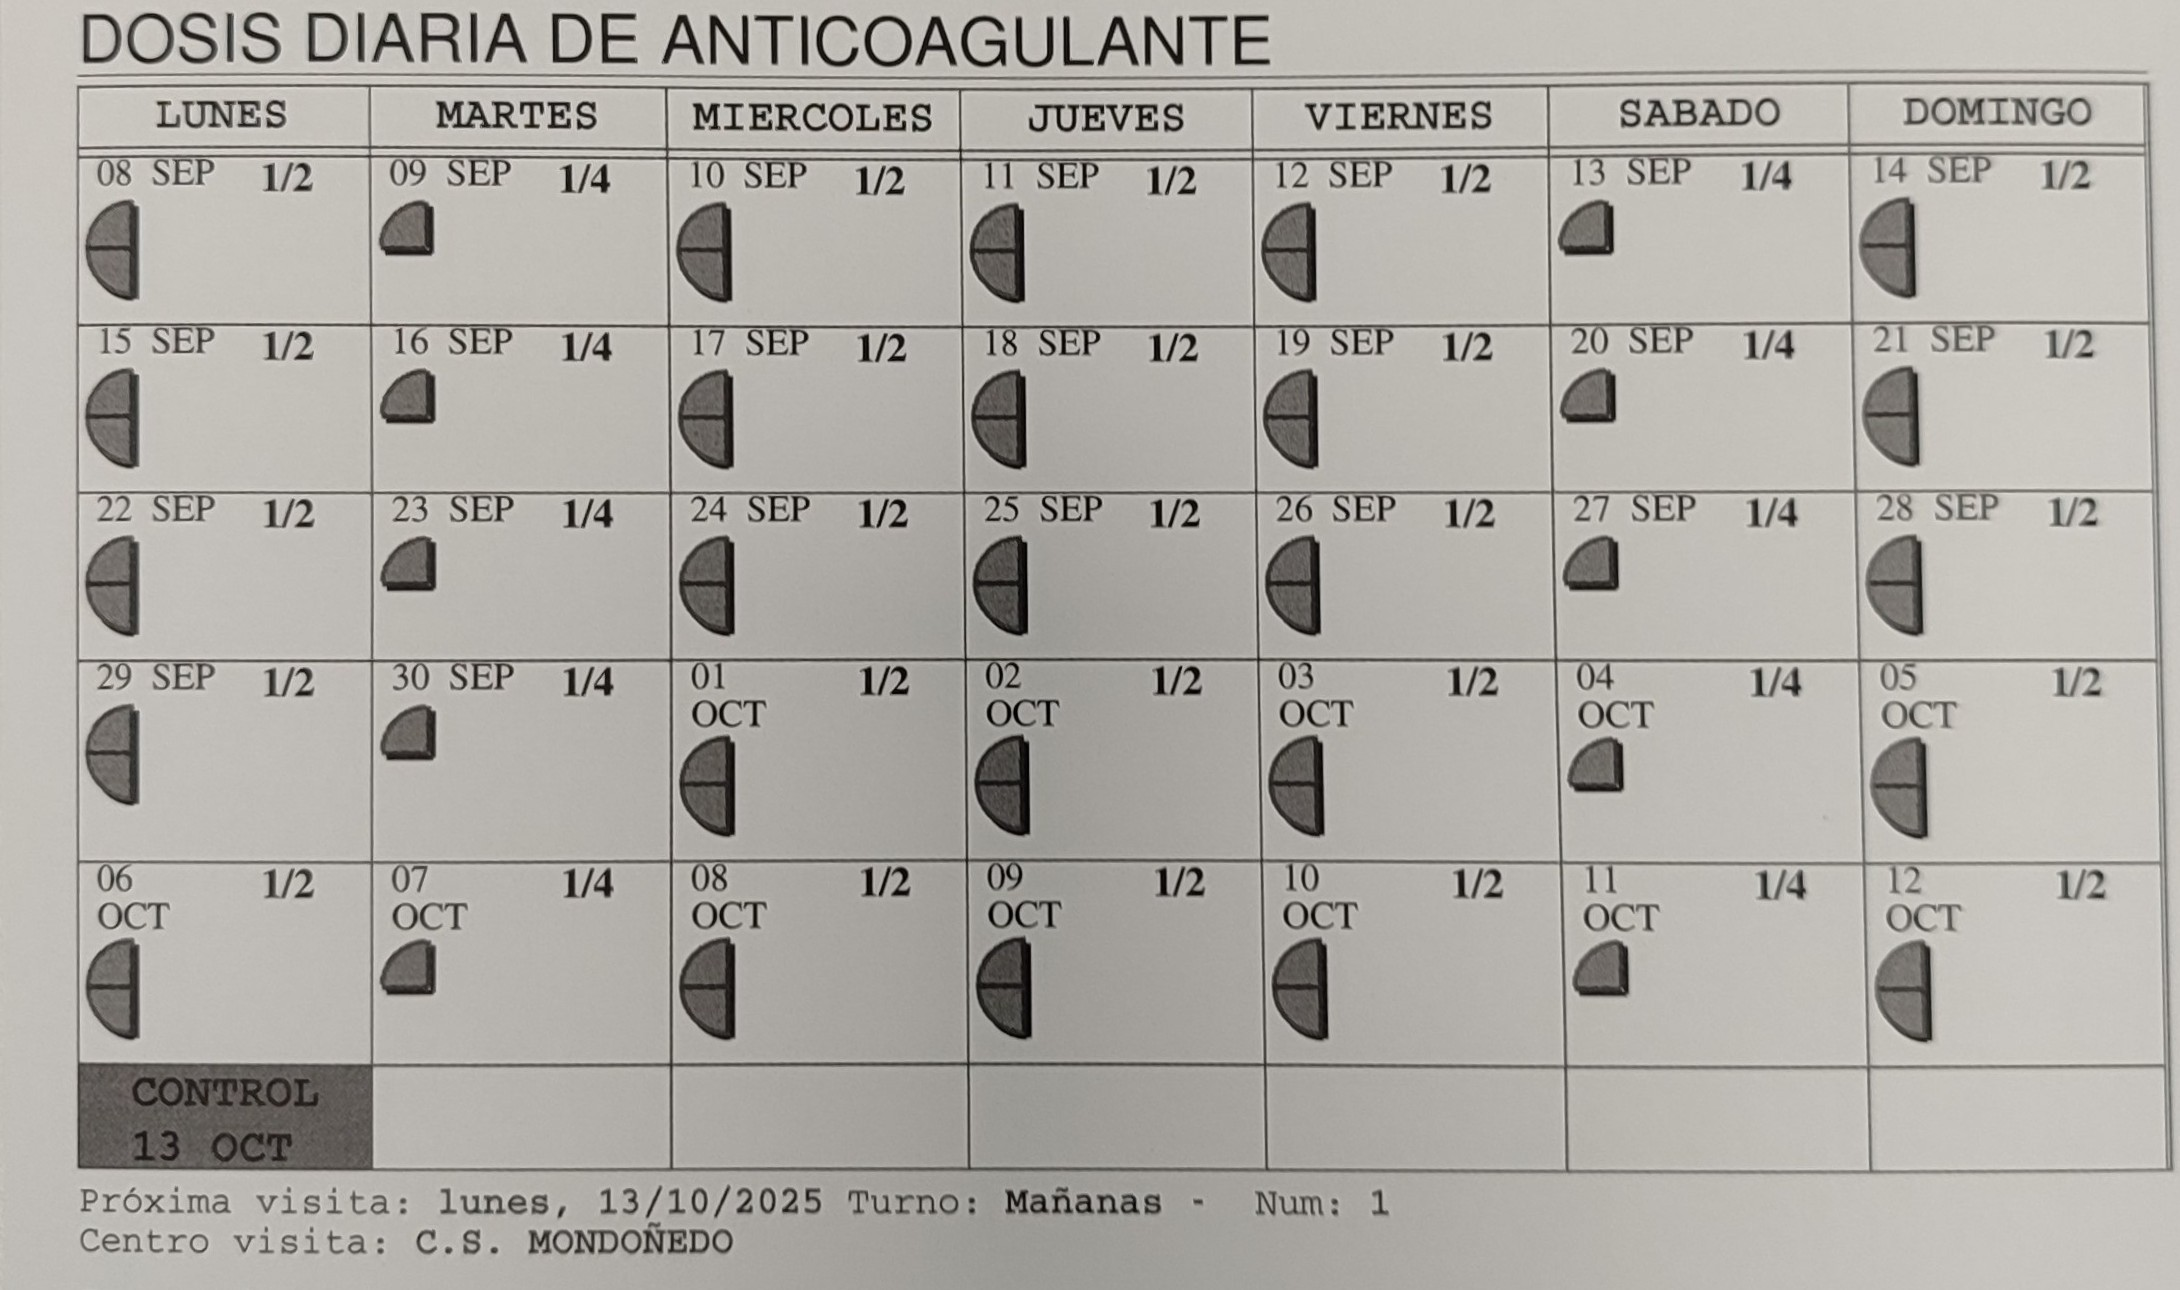
\includegraphics[width=0.65\textwidth]{imaxes/06-Procesamento automático das follas de tratamento/mlkit-f01n-pauta.jpg}
    \caption{Fragmento dunha folla escaneada empregada na avaliación do
    modelo estándar de Tesseract.}
    \label{fig:tesseract-estandar-f01}
\end{figure}

\begin{lstlisting}[
    frame=single,
    rulecolor=\color{gray!60},
    backgroundcolor=\color{gray!5},
    basicstyle=\ttfamily\scriptsize,
    caption={Fragmento da saída do modelo estándar de Tesseract para unha das follas escaneadas},
    label={lst:tesseract-estandar-f04},
    captionpos=t,
    columns=fullflexible,
    keepspaces=true
]
LUNES MARTES MIERCOLES JUEVES VIERNES SABADO |] DOMINGO
07 o [0 14 70 vo 10 va [1 o Ta
ENE ENE ENE ENE ENE
NO TOMAR a NO TOMAR NO TOMAR a
13 1/4 14 0 15 1/4
ENE ENE ENE
NO TOMAR
\end{lstlisting}

Noutros documentos o resultado foi aínda máis limitado. Na folla F02, por exemplo, Tesseract recoñeceu o título \textit{DOSIS DIARIA DE
ANTICOAGULANTE}, pero non recuperou o contido da táboa situada a continuación, pasando directamente á información da próxima visita.
Isto impide obter calquera asociación entre datas e doses para esa folla.

Os resultados non foron igualmente negativos en todos os documentos. Por exemplo, nalgunhas follas curtas Tesseract conseguiu conservar boa parte dunha fila da pauta. Porén, esta variabilidade entre documentos impide asumir que a mesma estratexia vaia proporcionar unha saída fiable para o conxunto de follas de tratamento.

Dado que estas limitacións apareceron xa nas follas escaneadas, non se considerou necesario estender a avaliación do modelo estándar a fotografías tomadas en diferentes condicións de captura. Os erros observados nas condicións máis favorables resultaban suficientes para descartar este modelo como solución directa. Estes resultados motivaron a realización de probas cun modelo de Tesseract adestrado especificamente para este tipo de documentos.

\subsubsection{Modelo personalizado}

O adestramento do modelo \textit{sintromv2} mostrou unha redución progresiva da taxa de erro ao longo do proceso. Como se observa na
Figura~\ref{fig:tesseract-sintromv2-adestramento}, o BCER pasou de valores próximos ao 39\,\% nas primeiras iteracións ata alcanzar un mínimo do \textbf{10,878\,\%}.

\begin{figure}[htbp]
    \centering
    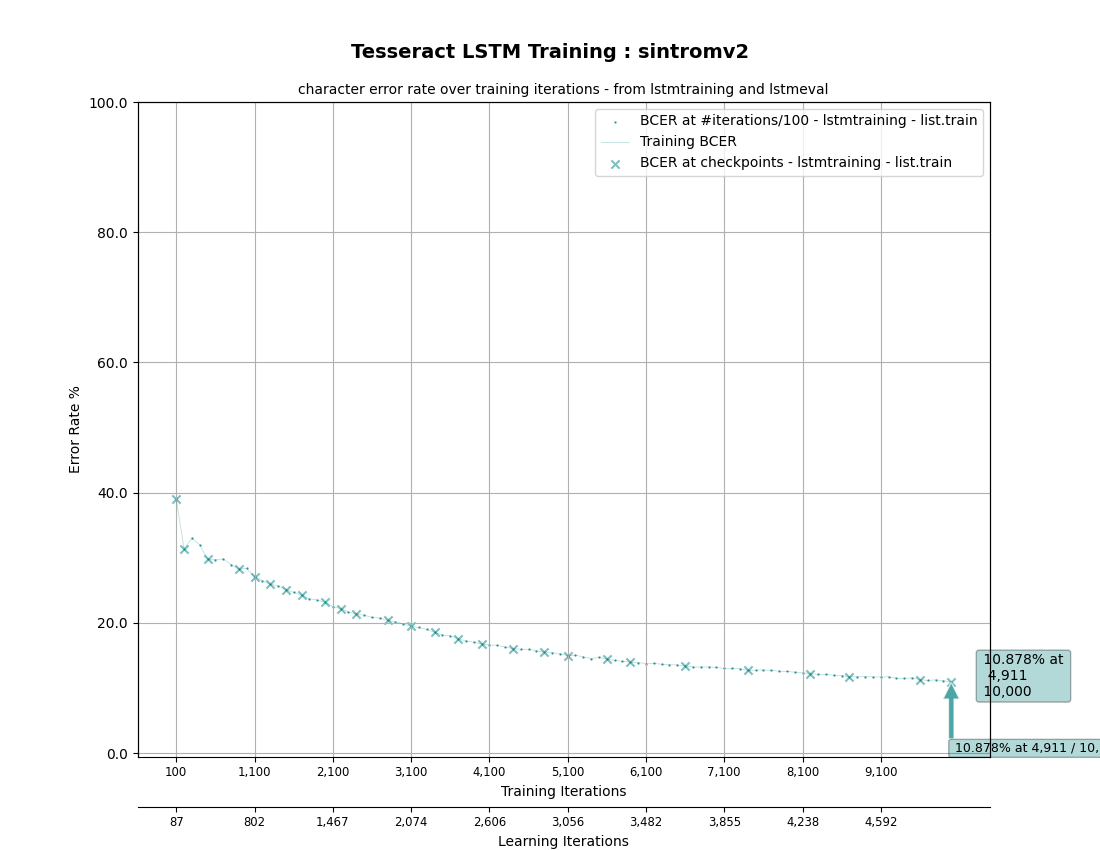
\includegraphics[width=0.75\textwidth]
    {imaxes/06-Procesamento automático das follas de tratamento/sintromv2.plot_cer.png}
    \caption{Evolución do BCER durante o adestramento do modelo
    \textit{sintromv2}.}
    \label{fig:tesseract-sintromv2-adestramento}
\end{figure}

O proceso completou as \textbf{10\,000 iteracións} empregadas por defecto por \textit{tesstrain} e obtivo o mellor resultado na
\textbf{iteración 4\,911}, cun BCER do \textbf{10,878\,\%} e un BWER do \textbf{20,409\,\%}. O punto de control correspondente a este resultado foi empregado para xerar o modelo final \textit{sintromv2}.

Seguindo a distribución indicada anteriormente, a avaliación realizouse sobre as follas \textbf{F09, F10 e F11}, que non foran empregadas durante o adestramento. As tres procesáronse nas catro condicións de captura definidas: imaxe escaneada, iluminación normal, menor iluminación e maior distancia.

Nas imaxes escaneadas observouse unha mellora respecto ao modelo estándar, especialmente no recoñecemento das fraccións empregadas para representar as doses. Un exemplo pode verse na folla F11, mostrada na  Figura~\ref{fig:tesseract-comparacion-f11}.

\begin{figure}[htbp]
\centering

\begin{minipage}[t]{0.48\textwidth}
\centering
\textbf{Modelo estándar}

\begin{lstlisting}[
    frame=single,
    rulecolor=\color{gray!60},
    backgroundcolor=\color{gray!5},
    basicstyle=\ttfamily\tiny,
    escapeinside={(*}{*)},
    columns=fullflexible,
    keepspaces=true
]
27 (*\textcolor{red}{12}*) 28 (*\textcolor{red}{12}*) 29 (*\textcolor{red}{12}*)
30 1/2 31 1/2 01 1/4
MAR MAR MAR MAR MAR ABR

02 (*\textcolor{red}{12}*) 03 (*\textcolor{red}{12}*) 04 (*\textcolor{red}{12}*)
ABR ABR ABR
\end{lstlisting}

\end{minipage}
\hfill
\begin{minipage}[t]{0.48\textwidth}
\centering
\textbf{Modelo \textit{sintromv2}}

\begin{lstlisting}[
    frame=single,
    rulecolor=\color{gray!60},
    backgroundcolor=\color{gray!5},
    basicstyle=\ttfamily\tiny,
    escapeinside={(*}{*)},
    columns=fullflexible,
    keepspaces=true
]
27 (*\textcolor{red}{1/2}*) 28 (*\textcolor{red}{1/2}*) 29 (*\textcolor{red}{1/2}*)
30 1/2 31 1/2 01 1/4
MAR MAR MAR MAR MAR ABR

02 (*\textcolor{red}{1/2}*) 03 (*\textcolor{red}{1/2}*) 04 (*\textcolor{red}{1/2}*)
ABR ABR ABR
\end{lstlisting}

\end{minipage}

\caption{Comparación dun fragmento da folla F11 co modelo estándar e co
modelo personalizado de Tesseract. En vermello destácanse algunhas das
fraccións corrixidas polo modelo \textit{sintromv2}.}
\label{fig:tesseract-comparacion-f11}
\end{figure}

A mellora non eliminou, con todo, os problemas de recoñecemento. Nas follas F09 e F10 continuaron aparecendo modificacións nas datas e perda da estrutura da táboa. Por exemplo, en F10 obtivéronse valores como \textit{068/09/2025} en lugar de \textit{08/09/2025} ou \textit{13/10/2023} en lugar de \textit{13/10/2025}, ao mesmo tempo que os elementos da pauta aparecían parcialmente desordenados.

Ao empregar fotografías, o comportamento empeorou. Mesmo con iluminación normal producíronse perdas importantes na táboa de doses; por exemplo, nunha das capturas de F10 recoñeceuse correctamente boa parte do texto xeral e a dose semanal, pero da pauta diaria practicamente só se conservaron os encabezados \textit{VIERNES} e \textit{DOMINGO}. Nas fotografías con menor iluminación e nas tomadas desde unha maior distancia a degradación foi aínda maior, chegando a obterse saídas nas que gran parte do texto e da estrutura do documento resultaban inintelixibles.

En conxunto, o adestramento específico permitiu mellorar o recoñecemento de determinados elementos, especialmente das fraccións. Porén, seguiron producíndose erros nas datas, nas doses e na organización da táboa, que se fixeron máis acusados ao empeorar as condicións de captura. Estes resultados impedían garantir unha reconstrución suficientemente fiable da pauta, polo que Tesseract foi descartado como solución principal para a extracción automática.

\subsection{Resultados de Azure AI Document Intelligence}

A avaliación de Azure AI Document Intelligence realizouse comparando os dous modelos personalizados adestrados, \textit{Template} e \textit{Neural}. Primeiro analizáronse as métricas proporcionadas ao finalizar o adestramento e, posteriormente, avaliáronse ambos modelos sobre as follas reservadas para as probas.

No modelo \textit{Template}, mostrado na Figura~\ref{fig:azure-metricas-template}, Azure proporciona unha estimación da precisión para cada un dos campos definidos.Os valores foron elevados na maior parte dos campos: 99,50\,\% para \textit{fecha visita}, \textit{inr}, \textit{farmaco oral} e \textit{prox visit}, 98,80\,\% para \textit{DOSE} e 94,70\,\% para \textit{RUV}. Os valores máis baixos corresponden a \textit{dosis semanal} e \textit{centro visita}, cun 87,50\,\%, e a \textit{turno}, cun 62,50\,\%. . Non obstante, estes campos teñen unha relevancia secundaria dentro da aplicación, xa que non afectan ao procesamento principal. En consecuencia, aínda que estes resultados son inferiores aos do resto dos campos, non representan un impacto significativo sobre o rendemento global do sistema.

%Bibliografía de azure  e poñer unha nota ou algo
No modelo \textit{Neural}, Azure Document Intelligence non proporciona puntuacións de precisión por campo durante o adestramento, polo que estes valores aparecen sen informar no Studio. Isto responde ao propio funcionamento deste tipo de modelo e non indica un erro no proceso de adestramento.

\begin{figure}[htbp]
    \centering
    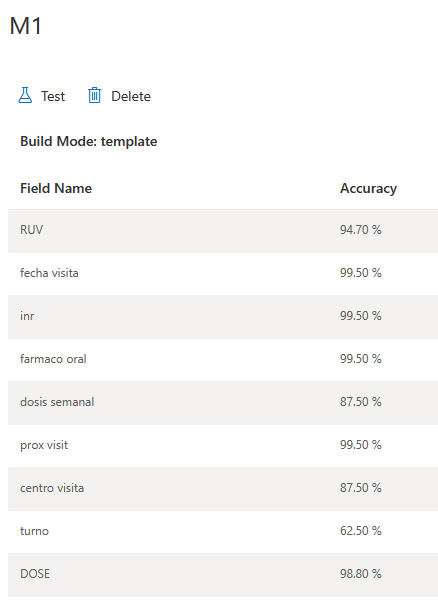
\includegraphics[width=0.4\textwidth]
    {imaxes/06-Procesamento automático das follas de tratamento/ResultM1.png}
    \caption{Precisión por campo mostrada por Azure Document Intelligence
    Studio para o modelo \textit{Template}.}
    \label{fig:azure-metricas-template}
\end{figure}


Nas probas sobre documentos non vistos, ambos modelos conseguiron recuperar correctamente numerosos campos individuais, como o INR, fármaco oral ou a data da visita. A principal diferenza apareceu na extracción da pauta diaria. O modelo \textit{Template} conservou de forma moito máis estable a agrupación dos días e das doses dentro das filas da táboa, mentres que o modelo \textit{Neural} fragmentou con frecuencia estes elementos en rexistros separados.

A plataforma de Azure devolve a información extraída nun documento con formato JSON para que poida ser consumido. O problema subxacente desta mala lectura visual é que o JSON resultante herda todo este caos. Ao non seguir un patrón predicible na súa resposta (nalgúns casos o JSON devolve a data e a dose xuntas, noutros devólveas separadas en distintas filas do obxecto …), resulta practicamente imposible deseñar unha lóxica de extracción que sexa capaz de recoller a información correcta para o día adecuado de forma robusta e automática

Un exemplo representativo desta diferenza pode observarse na folla F10 con iluminación normal. Como se mostra na Figura~\ref{fig:azure-comparacion-f10n}, o modelo \textit{Template} mantén nun mesmo rexistro os valores correspondentes aos sete días da semana. No modelo \textit{Neural}, pola contra, parte das datas e das doses son separadas en rexistros diferentes. Por exemplo, \textit{14 OCT} aparece separado da súa dose \textit{1/4}, dificultando a reconstrución directa da relación entre ambos elementos.

% Primeiro bloque (Páxina 1)
\begin{figure}[htbp]
    \centering
    
    % Primeira imaxe: Aumentamos o tamaño ao 90% do ancho do texto (\textwidth)
    \begin{subfigure}[t]{0.9\textwidth}
        \centering
        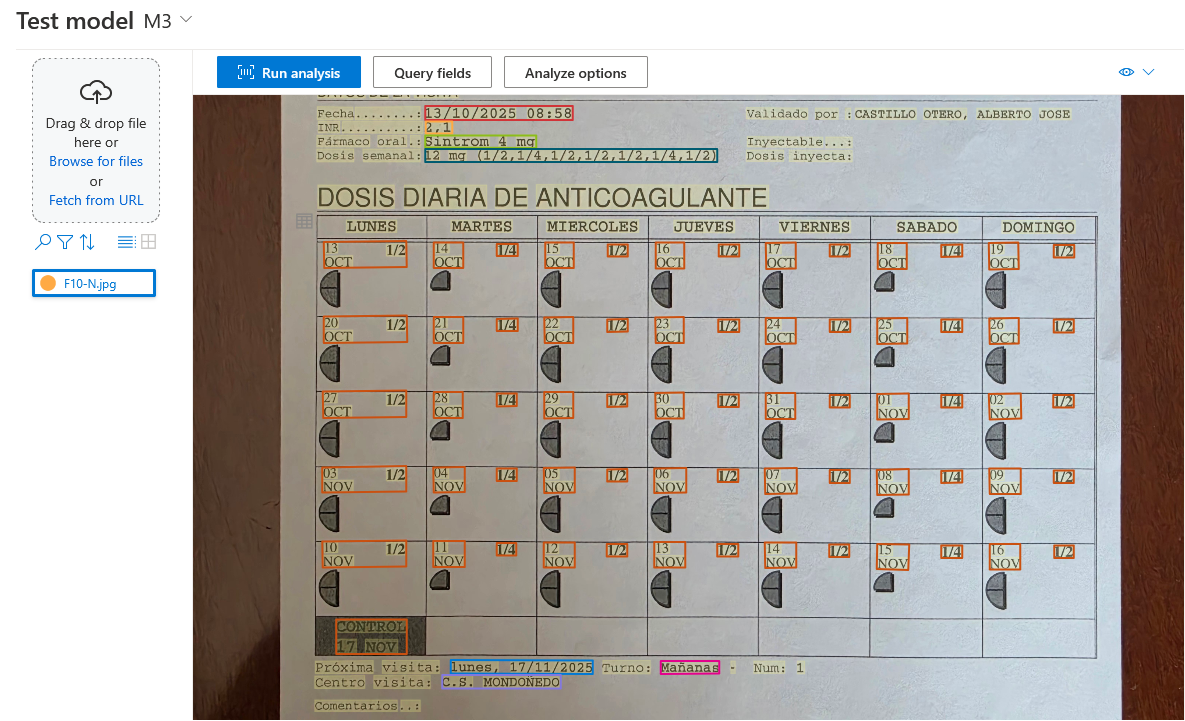
\includegraphics[width=\linewidth]{imaxes/06-Procesamento automático das follas de tratamento/azure-f10n-neural.png}
        \caption{Modelo \textit{Neural}.}
    \end{subfigure}
    
    \vspace{0.5cm} % Engadimos espazo vertical en lugar de \hfill
    
    % Segunda imaxe
    \begin{subfigure}[t]{0.9\textwidth}
        \centering
        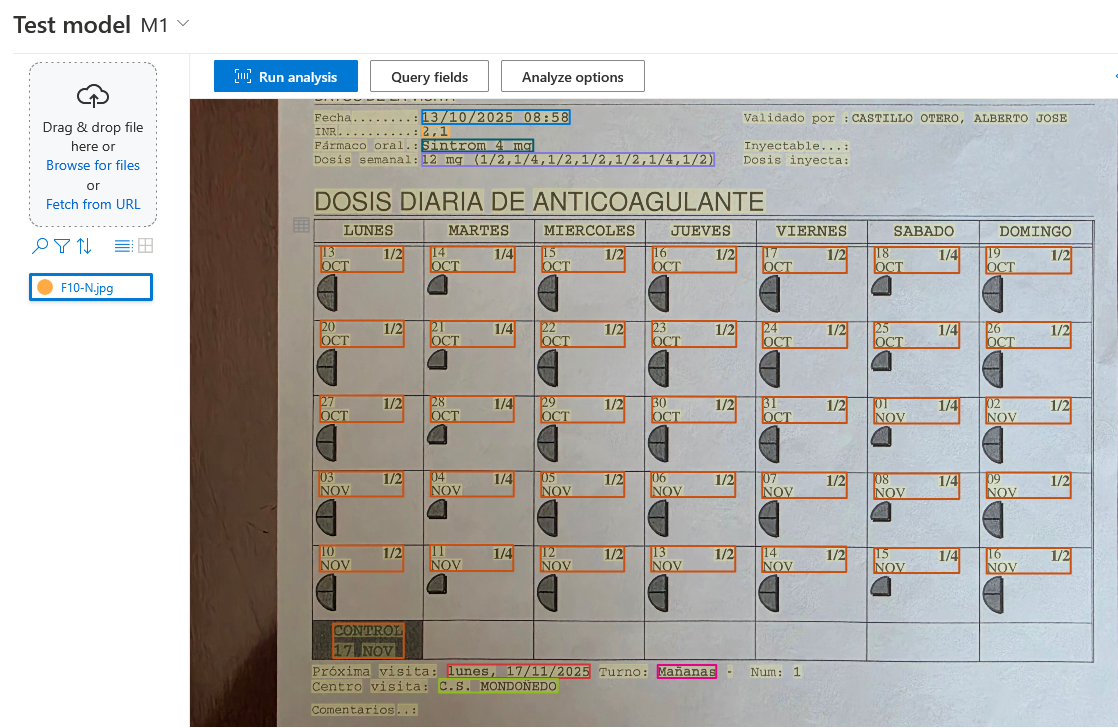
\includegraphics[width=\linewidth]{imaxes/06-Procesamento automático das follas de tratamento/azure-f10n-template.png}
        \caption{Modelo \textit{Template}.}
    \end{subfigure}

    \caption{Comparación da extracción da pauta da folla F10 con iluminación normal mediante os modelos \textit{Neural} e \textit{Template} (Parte 1).}
    \label{fig:azure-comparacion-f10n-1}
\end{figure}

% Segundo bloque (Páxina 2 ou a seguinte dispoñible)
\begin{figure}[htbp]
    \ContinuedFloat % <--- ISTO É A CLAVE: Dille a LaTeX que é a mesma figura que a anterior
    \centering
    
    % Terceira imaxe
    \begin{subfigure}[t]{0.9\textwidth}
        \centering
        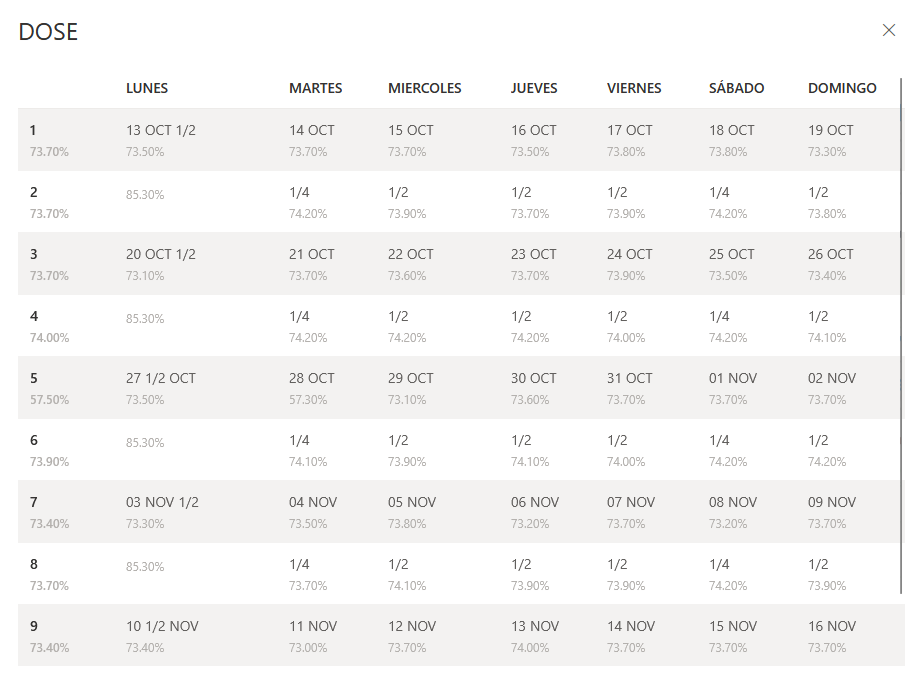
\includegraphics[width=\linewidth]{imaxes/06-Procesamento automático das follas de tratamento/azure-f10n-neural-taboa.png}
        \caption{Modelo \textit{Neural} (Táboas).}
    \end{subfigure}
    
    \vspace{0.5cm}
    
    % Cuarta imaxe
    \begin{subfigure}[t]{0.9\textwidth}
        \centering
        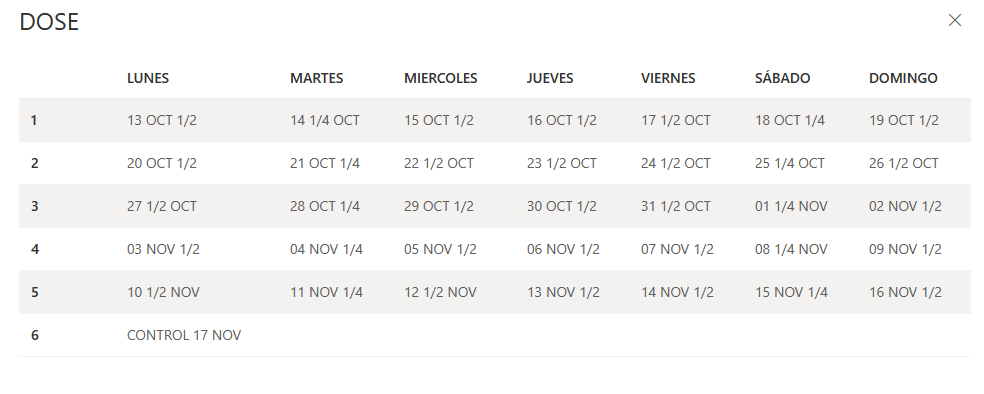
\includegraphics[width=\linewidth]{imaxes/06-Procesamento automático das follas de tratamento/azure-f10n-template-taboa.png}
        \caption{Modelo \textit{Template} (Táboas).}
    \end{subfigure}

    \caption{Comparación da extracción da pauta da folla F10 con iluminación normal mediante os modelos \textit{Neural} e \textit{Template} (Continuación).}
    \label{fig:azure-comparacion-f10n} % Esta é a etiqueta xeral que debes usar para referenciala no texto
\end{figure}

O modelo \textit{Template} non estivo exento de erros. Por exemplo, na folla F09 o campo \textit{turno} foi asociado incorrectamente co valor \textit{C.S. MONDOÑEDO}, mentres que o modelo \textit{Neural} recuperou correctamente \textit{Mañanas}.  Este resultado é coherente coa menor precisión obtida por este campo durante o adestramento do modelo \textit{Template}.


Nas condicións con menor iluminación, a cela de control resultou máis difícil de extraer correctamente debido ao sombreado escuro da propia cela, sobre o que se representan caracteres tamén escuros. Por exemplo, a entrada \textit{CONTROL 05 ABR} foi devolta unicamente como \textit{CONTROL}, perdéndose a data asociada.Esta perda non supón unha limitación práctica para
a aplicación, xa que a data do seguinte control pode obterse tamén a partir do campo \textit{prox visit}. Este campo presentou unha precisión do 99,50\,\% no modelo \textit{Template} e foi extraído correctamente en todas as probas realizadas.

En conxunto, ambos modelos permitiron recuperar unha parte importante da información das follas e mostraron un bo comportamento nos campos individuais. As principais diferenzas apareceron na estrutura da pauta diaria, onde o modelo \textit{Template} conservou de maneira máis consistente a asociación entre cada data e a súa dose. Aínda que se detectaron erros puntuais,
especialmente nas condicións de captura menos favorables, os resultados obtidos favoreceron este modelo para o procesamento estruturado das follas.


